% Created by tikzDevice version 0.12.6 on 2026-08-03 04:29:03
% !TEX encoding = UTF-8 Unicode
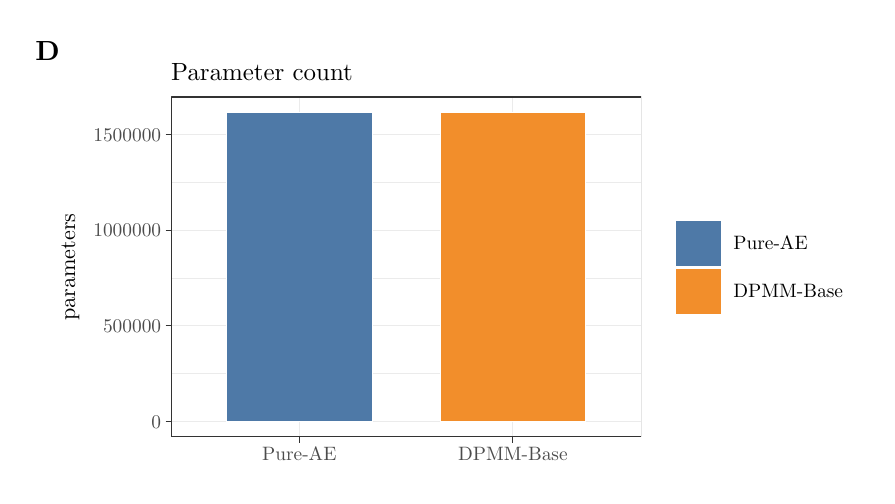
\begin{tikzpicture}[x=1pt,y=1pt]
\definecolor{fillColor}{RGB}{255,255,255}
\path[use as bounding box,fill=fillColor,fill opacity=0.00] (0,0) rectangle (303.38,161.83);
\begin{scope}
\path[clip] (  0.79,  1.74) rectangle (302.59,160.09);
\definecolor{drawColor}{RGB}{255,255,255}
\definecolor{fillColor}{RGB}{255,255,255}

\path[draw=drawColor,line width= 0.4pt,line join=round,line cap=round,fill=fillColor] (  0.79,  1.74) rectangle (302.59,160.09);
\end{scope}
\begin{scope}
\path[clip] ( 51.83, 13.93) rectangle (221.66,136.79);
\definecolor{fillColor}{RGB}{255,255,255}

\path[fill=fillColor] ( 51.83, 13.93) rectangle (221.66,136.79);
\definecolor{drawColor}{gray}{0.92}

\path[draw=drawColor,line width= 0.2pt,line join=round] ( 51.83, 36.80) --
	(221.66, 36.80);

\path[draw=drawColor,line width= 0.2pt,line join=round] ( 51.83, 71.37) --
	(221.66, 71.37);

\path[draw=drawColor,line width= 0.2pt,line join=round] ( 51.83,105.94) --
	(221.66,105.94);

\path[draw=drawColor,line width= 0.4pt,line join=round] ( 51.83, 19.52) --
	(221.66, 19.52);

\path[draw=drawColor,line width= 0.4pt,line join=round] ( 51.83, 54.09) --
	(221.66, 54.09);

\path[draw=drawColor,line width= 0.4pt,line join=round] ( 51.83, 88.66) --
	(221.66, 88.66);

\path[draw=drawColor,line width= 0.4pt,line join=round] ( 51.83,123.23) --
	(221.66,123.23);

\path[draw=drawColor,line width= 0.4pt,line join=round] ( 98.15, 13.93) --
	( 98.15,136.79);

\path[draw=drawColor,line width= 0.4pt,line join=round] (175.34, 13.93) --
	(175.34,136.79);
\definecolor{drawColor}{RGB}{255,255,255}
\definecolor{fillColor}{RGB}{78,121,167}

\path[draw=drawColor,line width= 0.3pt,fill=fillColor] ( 71.90, 19.52) rectangle (124.39,131.21);
\definecolor{fillColor}{RGB}{242,142,43}

\path[draw=drawColor,line width= 0.3pt,fill=fillColor] (149.10, 19.52) rectangle (201.59,131.21);
\definecolor{drawColor}{gray}{0.20}

\path[draw=drawColor,line width= 0.4pt,line join=round,line cap=round] ( 51.83, 13.93) rectangle (221.66,136.79);
\end{scope}
\begin{scope}
\path[clip] (  0.00,  0.00) rectangle (303.38,161.83);
\definecolor{drawColor}{gray}{0.30}

\node[text=drawColor,anchor=base east,inner sep=0pt, outer sep=0pt, scale=  0.70] at ( 48.23, 17.11) {0};

\node[text=drawColor,anchor=base east,inner sep=0pt, outer sep=0pt, scale=  0.70] at ( 48.23, 51.68) {500000};

\node[text=drawColor,anchor=base east,inner sep=0pt, outer sep=0pt, scale=  0.70] at ( 48.23, 86.25) {1000000};

\node[text=drawColor,anchor=base east,inner sep=0pt, outer sep=0pt, scale=  0.70] at ( 48.23,120.82) {1500000};
\end{scope}
\begin{scope}
\path[clip] (  0.00,  0.00) rectangle (303.38,161.83);
\definecolor{drawColor}{gray}{0.20}

\path[draw=drawColor,line width= 0.4pt,line join=round] ( 49.83, 19.52) --
	( 51.83, 19.52);

\path[draw=drawColor,line width= 0.4pt,line join=round] ( 49.83, 54.09) --
	( 51.83, 54.09);

\path[draw=drawColor,line width= 0.4pt,line join=round] ( 49.83, 88.66) --
	( 51.83, 88.66);

\path[draw=drawColor,line width= 0.4pt,line join=round] ( 49.83,123.23) --
	( 51.83,123.23);
\end{scope}
\begin{scope}
\path[clip] (  0.00,  0.00) rectangle (303.38,161.83);
\definecolor{drawColor}{gray}{0.20}

\path[draw=drawColor,line width= 0.4pt,line join=round] ( 98.15, 11.93) --
	( 98.15, 13.93);

\path[draw=drawColor,line width= 0.4pt,line join=round] (175.34, 11.93) --
	(175.34, 13.93);
\end{scope}
\begin{scope}
\path[clip] (  0.00,  0.00) rectangle (303.38,161.83);
\definecolor{drawColor}{gray}{0.30}

\node[text=drawColor,anchor=base,inner sep=0pt, outer sep=0pt, scale=  0.70] at ( 98.15,  5.51) {Pure-AE};

\node[text=drawColor,anchor=base,inner sep=0pt, outer sep=0pt, scale=  0.70] at (175.34,  5.51) {DPMM-Base};
\end{scope}
\begin{scope}
\path[clip] (  0.00,  0.00) rectangle (303.38,161.83);
\definecolor{drawColor}{RGB}{0,0,0}

\node[text=drawColor,rotate= 90.00,anchor=base,inner sep=0pt, outer sep=0pt, scale=  0.80] at ( 17.12, 75.36) {parameters};
\end{scope}
\begin{scope}
\path[clip] (  0.00,  0.00) rectangle (303.38,161.83);
\definecolor{fillColor}{RGB}{255,255,255}

\path[fill=fillColor] (229.66, 54.02) rectangle (300.59, 96.71);
\end{scope}
\begin{scope}
\path[clip] (  0.00,  0.00) rectangle (303.38,161.83);
\definecolor{fillColor}{RGB}{255,255,255}

\path[fill=fillColor] (233.66, 75.36) rectangle (251.01, 92.71);
\definecolor{drawColor}{RGB}{255,255,255}
\definecolor{fillColor}{RGB}{78,121,167}

\path[draw=drawColor,line width= 0.3pt,fill=fillColor] (234.02, 75.72) rectangle (250.65, 92.35);
\end{scope}
\begin{scope}
\path[clip] (  0.00,  0.00) rectangle (303.38,161.83);
\definecolor{fillColor}{RGB}{255,255,255}

\path[fill=fillColor] (233.66, 58.02) rectangle (251.01, 75.36);
\definecolor{drawColor}{RGB}{255,255,255}
\definecolor{fillColor}{RGB}{242,142,43}

\path[draw=drawColor,line width= 0.3pt,fill=fillColor] (234.02, 58.37) rectangle (250.65, 75.01);
\end{scope}
\begin{scope}
\path[clip] (  0.00,  0.00) rectangle (303.38,161.83);
\definecolor{drawColor}{RGB}{0,0,0}

\node[text=drawColor,anchor=base west,inner sep=0pt, outer sep=0pt, scale=  0.70] at (255.01, 81.62) {Pure-AE};
\end{scope}
\begin{scope}
\path[clip] (  0.00,  0.00) rectangle (303.38,161.83);
\definecolor{drawColor}{RGB}{0,0,0}

\node[text=drawColor,anchor=base west,inner sep=0pt, outer sep=0pt, scale=  0.70] at (255.01, 64.28) {DPMM-Base};
\end{scope}
\begin{scope}
\path[clip] (  0.00,  0.00) rectangle (303.38,161.83);
\definecolor{drawColor}{RGB}{0,0,0}

\node[text=drawColor,anchor=base west,inner sep=0pt, outer sep=0pt, scale=  0.90] at ( 51.83,142.78) {Parameter count};
\end{scope}
\begin{scope}
\path[clip] (  0.00,  0.00) rectangle (303.38,161.83);
\definecolor{drawColor}{RGB}{0,0,0}

\node[text=drawColor,anchor=base,inner sep=0pt, outer sep=0pt, scale=  1.00] at (  7.20,150.08) {\bfseries D};
\end{scope}
\end{tikzpicture}
